% ------------------------------------------------------------------------------
% TYPO3 CMS 6.2 LTS - What's New - Chapter "Backend veranderingen" (Dutch Version)
%
% @author	Christiaan Wiesenekker <cwiesenekker@gmail.com>
% @author	Ric van Westhreenen <ric.vanwesthreenen@typo3.org>
% @license	Creative Commons BY-NC-SA 3.0
% @link		http://typo3.org/download/release-notes/whats-new/
% @language	Dutch
% ------------------------------------------------------------------------------
% Chapter: Backend veranderingen
% ------------------------------------------------------------------------------

\section{Backend veranderingen}
\begin{frame}[fragile]
	\frametitle{Backend veranderingen}

	\begin{center}\huge{Hoofdstuk 3:}\end{center}
	\begin{center}\huge{\color{typo3darkgrey}\textbf{Backend veranderingen}}\end{center}

\end{frame}

% ------------------------------------------------------------------------------
% Autofocus
% ------------------------------------------------------------------------------
% http://forge.typo3.org/issues/49228

\begin{frame}[fragile]
	\frametitle{Backend veranderingen}
	\framesubtitle{Backend Login}

 	\begin{itemize}
		\item Autofocus op het veld: 'gebruikersnaam' tijdens de login\newline
			(HTML5 attibute: \texttt{autofocus="autofocus"})
	\end{itemize}

	\begin{figure}
		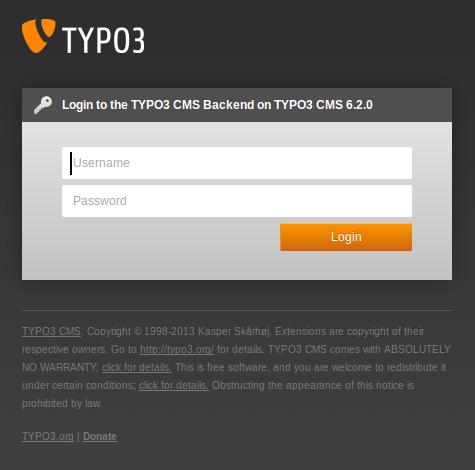
\includegraphics[width=0.4\linewidth]{Images/BackendChanges/BackendLogin.png}
	\end{figure}

\end{frame}

% ------------------------------------------------------------------------------
% Visual Appearance
% ------------------------------------------------------------------------------
% http://forge.typo3.org/issues/48376

\begin{frame}[fragile]
	\frametitle{Backend veranderingen}
	\framesubtitle{Grafische weergave}

	\begin{columns}[T]

		\begin{column}{.5\textwidth}
			\begin{itemize}
				\item Verhoogde gebruiksvriendelijkeheid door het verbeteren van de layout
				\item Margins tussen module items (linker kolom) verbeterd
				\item Gebaseerd op een 12px gird, welke is verhoogd
				\end{itemize}
		\end{column}

		\begin{column}{.5\textwidth}
			\begin{figure}\vspace*{-0.4cm}
				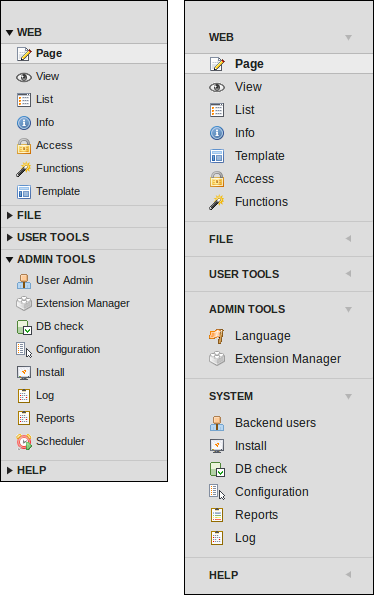
\includegraphics[width=0.6\linewidth]{Images/BackendChanges/VisualAppearance.png}
			\end{figure}
		\end{column}

	\end{columns}

\end{frame}

% ------------------------------------------------------------------------------
% Visual Appearance
% ------------------------------------------------------------------------------

\begin{frame}[fragile]
	\frametitle{Backend veranderingen}
	\framesubtitle{Grafische weergave}

	\begin{columns}[T]

		\begin{column}{.5\textwidth}

			\begin{itemize}
				\item Modules in de linker kolom geherstructureerd
				\item Module "ADMINTOOLS" verdeeld in twee delen:

					\begin{itemize}
						\item \textbf{ADMINTOOLS} ("Talen" and "Extensiemanager")
						\item \textbf{SYSTEEM} ('low-level tools', welke zelf geen onderdeel kunnen zijn in de paginaboom kolom)
					\end{itemize}

				\item Module "TypoScript-Help" verwijderd (verouderd)

			\end{itemize}

		\end{column}

		\begin{column}{.5\textwidth}
			\begin{figure}\vspace*{-0.4cm}
				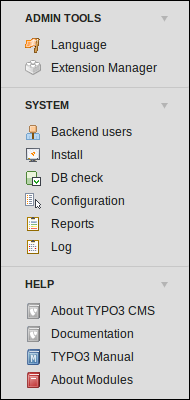
\includegraphics[width=0.35\linewidth]{Images/BackendChanges/AdminTools.png}
			\end{figure}
		\end{column}

	\end{columns}

\end{frame}

% ------------------------------------------------------------------------------
% Visual Appearance
% ------------------------------------------------------------------------------
% http://forge.typo3.org/issues/36017

\begin{frame}[fragile]
	\frametitle{Backend veranderingen}
	\framesubtitle{Grafische weergave}

	\begin{itemize}
		\item \texttt{<h1>}-koppen in het overzicht (rechterkolom) gebruiken het TYPO3 font "Share" consistent
	\end{itemize}

	\begin{figure}
		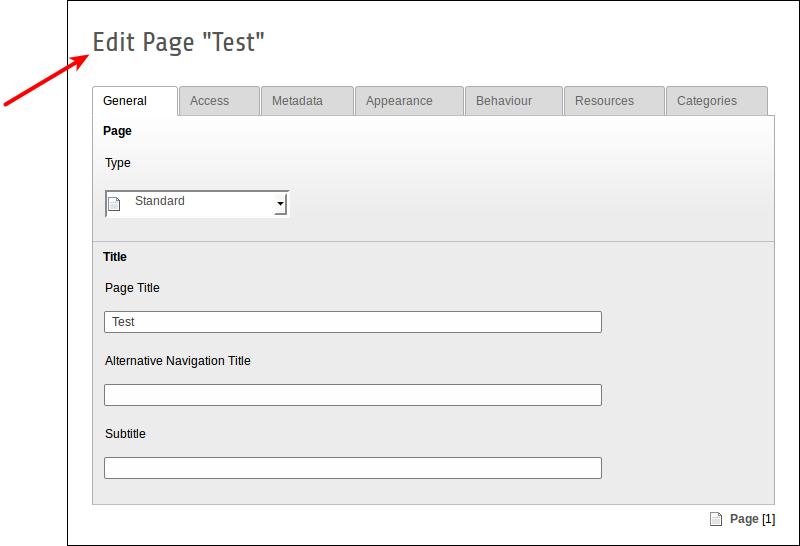
\includegraphics[width=0.6\linewidth]{Images/BackendChanges/ConsistantFont.png}
	\end{figure}

\end{frame}

% ------------------------------------------------------------------------------
% Visual Appearance
% ------------------------------------------------------------------------------
% http://forge.typo3.org/issues/41631

\begin{frame}[fragile]
	\frametitle{Backend veranderingen}
	\framesubtitle{Grafische weergave}

	\begin{itemize}
		\item Module "rapporten" heeft een nieuwe icoon
	\end{itemize}

	\begin{figure}
		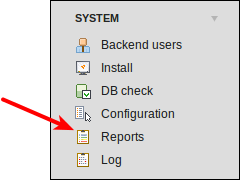
\includegraphics[width=0.35\linewidth]{Images/BackendChanges/ModuleReportsIcon.png}
	\end{figure}

\end{frame}

% ------------------------------------------------------------------------------
% Filelist: Drag&Drop File Upload
% ------------------------------------------------------------------------------
% http://forge.typo3.org/issues/47005

\begin{frame}[fragile]
	\frametitle{Backend veranderingen}
	\framesubtitle{Drag\&Drop File Upload}

	\begin{itemize}
		\item Vanaf TYPO3 6.1 is de Flash-uploader verwijderd
		\item HTML5 Drag\&Drop bestandsupload functionaliteit geimplementeerd in de bestandenlijst

	\end{itemize}

	\begin{figure}
		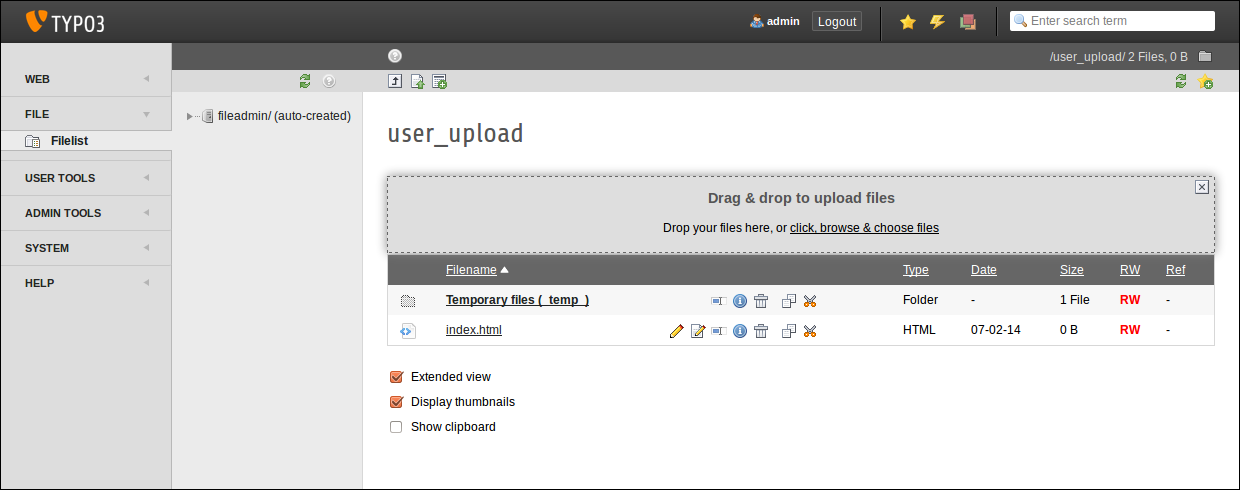
\includegraphics[width=0.95\linewidth]{Images/BackendChanges/DragDropFileUpload.png}
	\end{figure}

\end{frame}

% ------------------------------------------------------------------------------
% Drag&Drop File Upload Via Content Elements
% (slide added in March 2014)
% ------------------------------------------------------------------------------
%
%\begin{frame}[fragile]
%	\frametitle{Backend Changes}
%	\framesubtitle{Drag\&Drop File Upload (2)}
%
%	\begin{itemize}
%		\item ...and via content elements (button: "Select \& upload files")
%
%	\end{itemize}
%
%	\begin{figure}
%		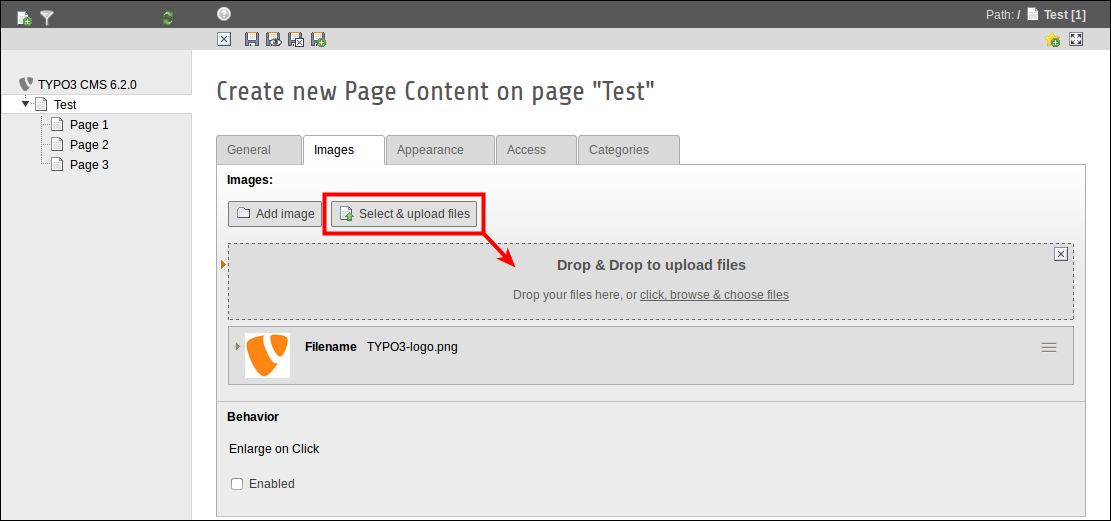
\includegraphics[width=0.95\linewidth]{Images/BackendChanges/SelectAndUploadFiles.png}
%	\end{figure}
%
%\end{frame}

% ------------------------------------------------------------------------------
% Backend Users
% ------------------------------------------------------------------------------
% http://forge.typo3.org/issues/43053

\begin{frame}[fragile]
	\frametitle{Backend veranderingen}
	\framesubtitle{Usability: Backend gebruikers beheer}

	\begin{itemize}
		\item Gebruikersnaam en echte naam worden getoond (eerste kolom in de lijst weergave)
		\item Klik op (gebruikers)naam om een gebruiker aan te passen 
		\item Verwijder-knop in de lijst weergave van de gebruikers

	\end{itemize}

	\begin{figure}
		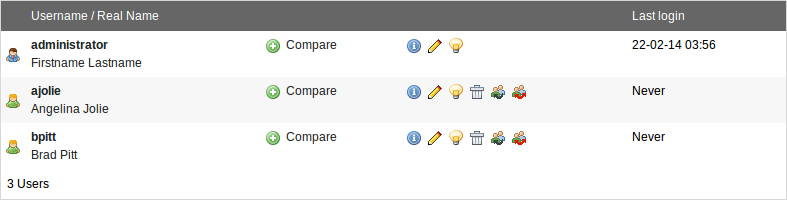
\includegraphics[width=0.95\linewidth]{Images/BackendChanges/BackendUserList.png}
	\end{figure}

\end{frame}

% ------------------------------------------------------------------------------
% Live Search
% ------------------------------------------------------------------------------
% http://forge.typo3.org/issues/35358

\begin{frame}[fragile]
	\frametitle{Backend veranderingen}
	\framesubtitle{Live zoeken}

	\begin{itemize}
		\item Toont de UID en de PID van de gevonden records bij een mouseover
		\item Wanneer na het zoeken het bewerk scherm weer is gesloten wordt de lijstweergave van de pagina getoond (en niet een lege pagina)
	\end{itemize}

	\begin{figure}
		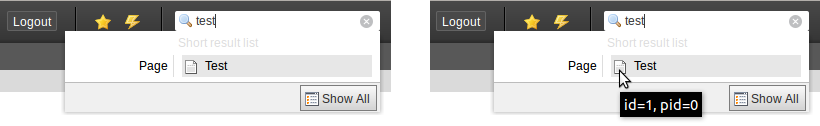
\includegraphics[width=0.8\linewidth]{Images/BackendChanges/LiveSearchTooltip.png}
	\end{figure}

\end{frame}

% ------------------------------------------------------------------------------
% Live Search
% ------------------------------------------------------------------------------

\begin{frame}[fragile]
	\frametitle{Backend veranderingen}
	\framesubtitle{Live Search}

	\begin{itemize}
		\item In TYPO3 < 6.2 werd voor paginas alleen rekening gehouden met de database velden \texttt{title} en \texttt{uid}
		\item In TYPO3 >= 6.2 kan het veld \texttt{alias} worden toegevoegd aan het zoeken \newline
			(vereist UserTSconfig: \texttt{options.pageTree.searchInAlias = 1})
	\end{itemize}

	\begin{figure}
		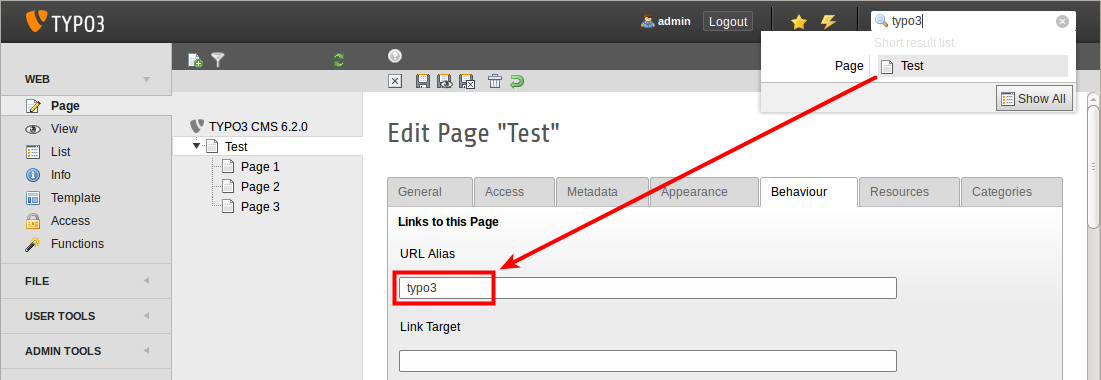
\includegraphics[width=0.95\linewidth]{Images/BackendChanges/LiveSearchInAlias.png}
	\end{figure}

\end{frame}

% ------------------------------------------------------------------------------
% File Abstraction Layer
% ------------------------------------------------------------------------------

\begin{frame}[fragile]
	\frametitle{Backend veranderingen}
	\framesubtitle{File Abstraction Layer}

	\begin{itemize}
		\item Bestandsnaam en titel worden getoond in de FAL element header
	\end{itemize}

	\begin{figure}
		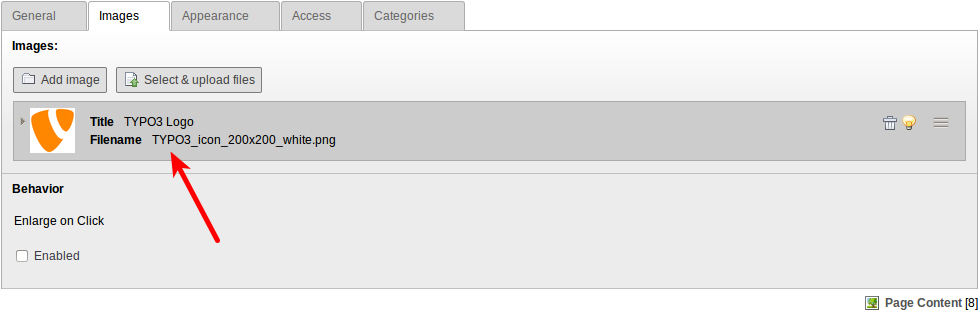
\includegraphics[width=0.95\linewidth]{Images/BackendChanges/FalTitleAndFilename.png}
	\end{figure}

\end{frame}

% ------------------------------------------------------------------------------
% File Abstraction Layer
% ------------------------------------------------------------------------------

\begin{frame}[fragile]
	\frametitle{Backend veranderingen}
	\framesubtitle{File Abstraction Layer (EXT:filemetadata)}

	\begin{itemize}
		\item EXT:filemetadata voegt een tab toe die zorgt voor het tonen van meta data(extensie is niet standaard geinstalleerd maar is wel aanwezig in de package)
	\end{itemize}

	\begin{figure}
		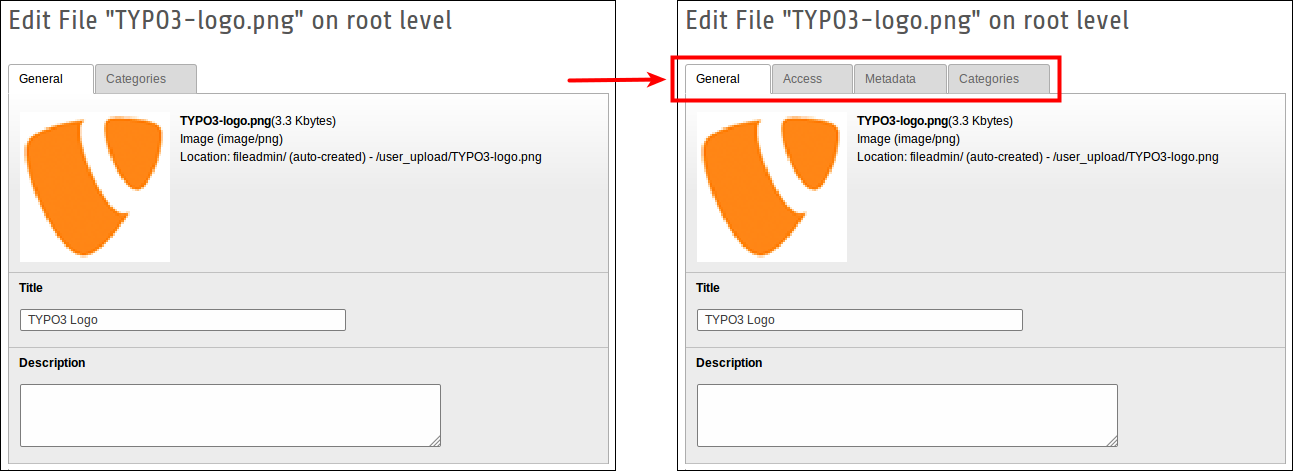
\includegraphics[width=0.95\linewidth]{Images/BackendChanges/FileMetaDataTabs.png}
	\end{figure}

\end{frame}

% ------------------------------------------------------------------------------
% File Abstraction Layer
% ------------------------------------------------------------------------------

\begin{frame}[fragile]
	\frametitle{Backend Changes}
	\framesubtitle{File Abstraction Layer (EXT:filemetadata)}

	\begin{figure}
		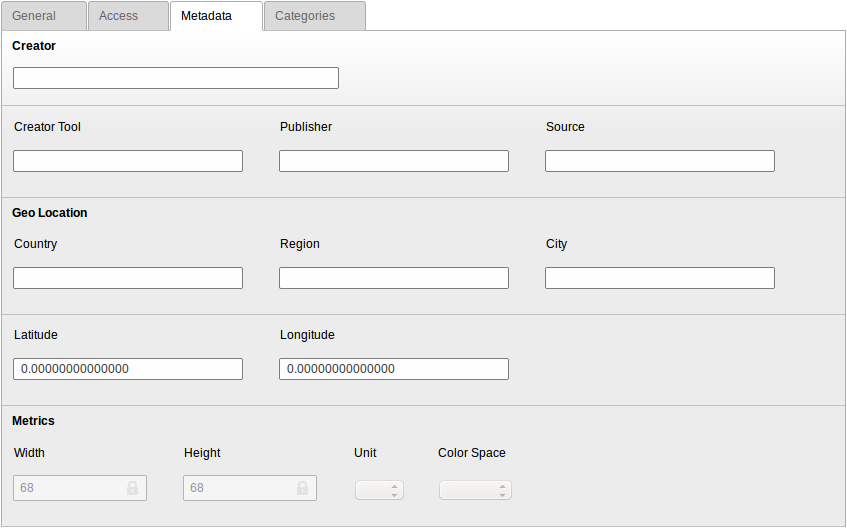
\includegraphics[width=0.8\linewidth]{Images/BackendChanges/FileMetaData.png}
	\end{figure}

\end{frame}

% ------------------------------------------------------------------------------
% File Abstraction Layer
% ------------------------------------------------------------------------------

\begin{frame}[fragile]
	\frametitle{Backend veranderingen}
	\framesubtitle{File Abstraction Layer}

	\begin{itemize}
		\item Het is nu mogelijk om FAL metadata te vertalen naar andere Frontend talen.
	\end{itemize}

	\begin{figure}
		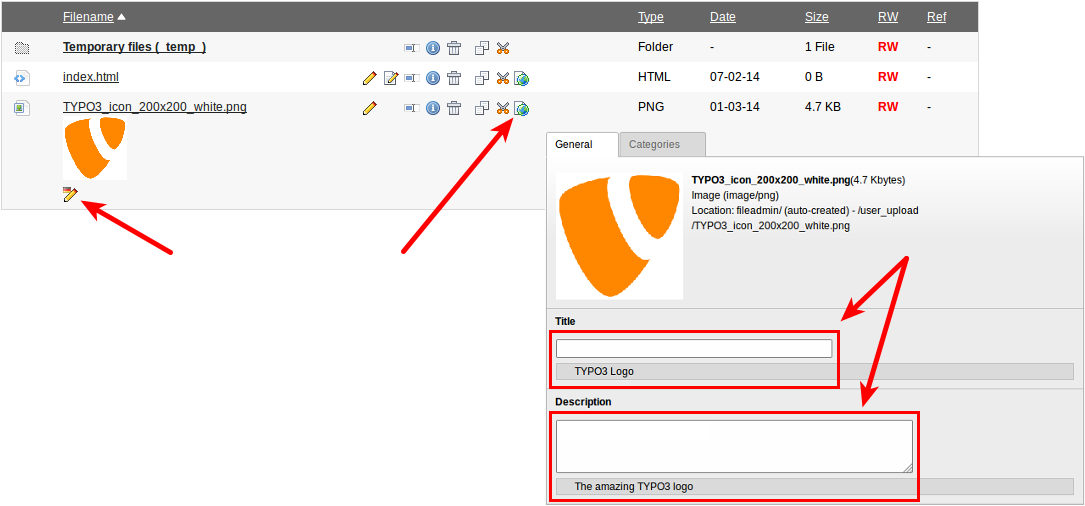
\includegraphics[width=0.95\linewidth]{Images/BackendChanges/FalTranslateMetaData.png}
	\end{figure}

\end{frame}

% ------------------------------------------------------------------------------
% Module: Documentation
% ------------------------------------------------------------------------------

\begin{frame}[fragile]
	\frametitle{Backend veranderingen}
	\framesubtitle{Module: Documentatie}

	\begin{columns}[T]

		\begin{column}{.5\textwidth}
			\begin{itemize}
				\item Module "Documentatie" staat BE gebruikers het toe om handleidingen te bekijken en te downloaden
				\item Nieuwe TYPO3 installaties laden deze module standaard
				\item Gebruik de Extensiemanager om de "Documentatie" te laden in een bijgewerkte TYPO3 installatie 
				\item De functie "Download documentatie", download de handleidingen(zie illustratie)
			\end{itemize}
		\end{column}

		\begin{column}{.5\textwidth}
			\begin{figure}\vspace*{-0.4cm}
				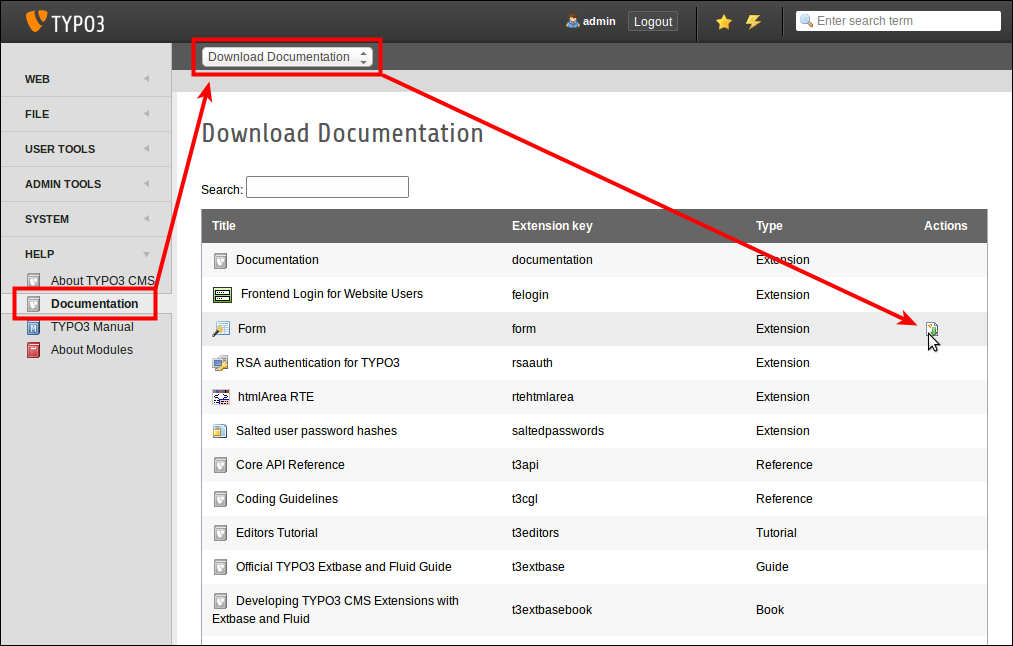
\includegraphics[width=1\linewidth]{Images/BackendChanges/DownloadDocumentation.png}
			\end{figure}
		\end{column}

	\end{columns}

\end{frame}

% ------------------------------------------------------------------------------
% Module: Documentation
% ------------------------------------------------------------------------------

\begin{frame}[fragile]
	\frametitle{Backend veranderingen}
	\framesubtitle{Module: Documentatie}

	\begin{itemize}
		\item Functie "Toon Documentatie" toont gedownloade handleidingen
	\end{itemize}

	\begin{figure}
		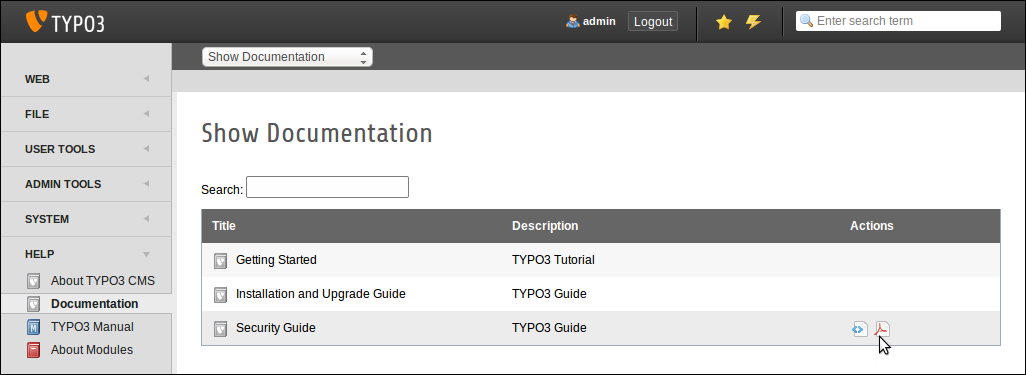
\includegraphics[width=0.95\linewidth]{Images/BackendChanges/ShowDocumentation.png}
	\end{figure}

\end{frame}

% ------------------------------------------------------------------------------
% Removed: TypoScript Help
% ------------------------------------------------------------------------------
% http://forge.typo3.org/issues/47931

\begin{frame}[fragile]
	\frametitle{Backend veranderingen}
	\framesubtitle{Verwijderd: TypoScript Help}

 	\begin{itemize}
		\item EXT:tsconfig\_help ("TSconfig Quick Reference") verwijderd\newline
			\small(achterhaalde informatie en niet onderhouden sinds TYPO3 4.1)
	\end{itemize}

	\begin{figure}
		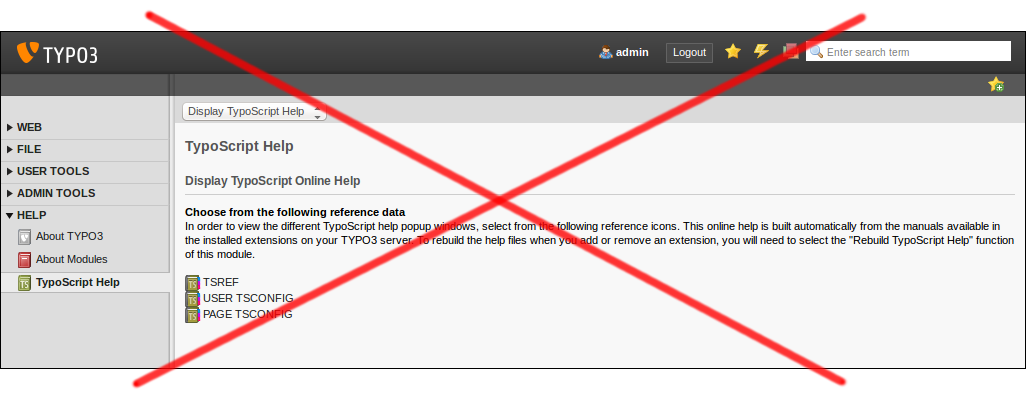
\includegraphics[width=0.95\linewidth]{Images/BackendChanges/TypoScriptHelpRemovedCrossed.png}
	\end{figure}

\end{frame}


% ------------------------------------------------------------------------------
% Scheduler
% ------------------------------------------------------------------------------

\begin{frame}[fragile]
	\frametitle{Backend veranderingen}
	\framesubtitle{Taakplanner}

	\begin{itemize}
		\item Verwijder taakplanner taken in het 'edit' scherm \newline
			(in TYPO3 < 6.2 was de verwijder optie alleen mogelijk via de lijstweergave)
	\end{itemize}

	\begin{figure}
		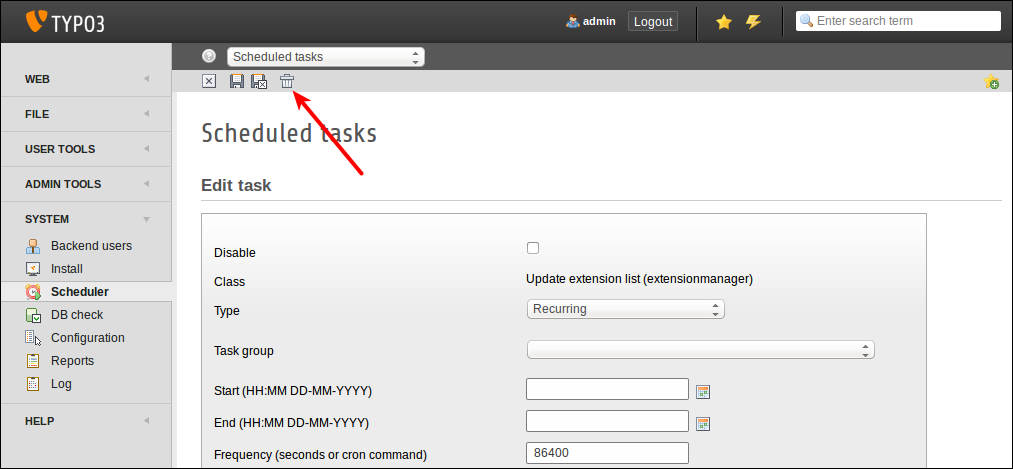
\includegraphics[width=0.95\linewidth]{Images/BackendChanges/DeleteSchedulerTaskInEditView.png}
	\end{figure}

\end{frame}

% ------------------------------------------------------------------------------
% Scheduler
% ------------------------------------------------------------------------------

\begin{frame}[fragile]
	\frametitle{Backend veranderingen}
	\framesubtitle{Taakplanner}

	\begin{itemize}
		\item Een omschrijving kan worden toegevoegd aan de taken en worden getoond als subheaders in de lijstweergave, of als tooltips (zie volgende slide)
	\end{itemize}

	\begin{figure}
		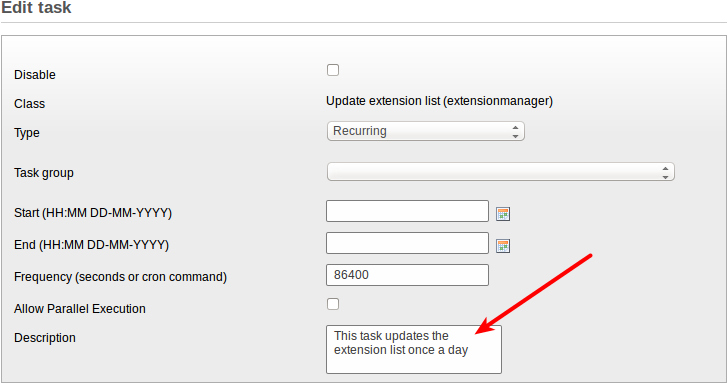
\includegraphics[width=0.7\linewidth]{Images/BackendChanges/SchedulerTaskDescription.png}
	\end{figure}

\end{frame}

% ------------------------------------------------------------------------------
% Scheduler
% ------------------------------------------------------------------------------

\begin{frame}[fragile]
	\frametitle{Backend veranderingen}
	\framesubtitle{Taakplanner}

	\begin{itemize}
		\item Taak omschrijving als  subheader\newline
			\small(dit moet nog worden geactiveerd via de extenstie configuratie)\normalsize
	\end{itemize}

	\begin{figure}
		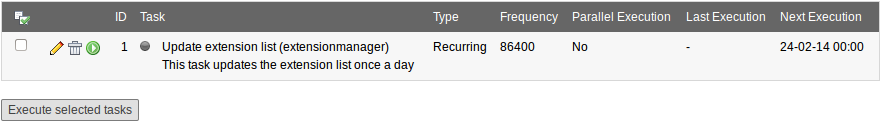
\includegraphics[width=0.95\linewidth]{Images/BackendChanges/SchedulerTaskDescriptionAsSubheader.png}
	\end{figure}

	\begin{itemize}
		\item Taak omschrijving als tooltip ("hover")
	\end{itemize}

	\begin{figure}
		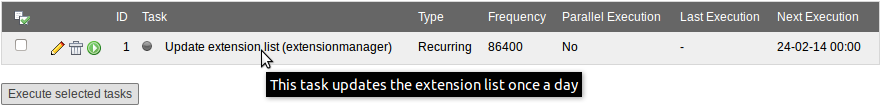
\includegraphics[width=0.95\linewidth]{Images/BackendChanges/SchedulerTaskDescriptionAsTooltip.png}
	\end{figure}

\end{frame}

% ------------------------------------------------------------------------------
% Scheduler
% ------------------------------------------------------------------------------

\begin{frame}[fragile]
	\frametitle{Backend veranderingen}
	\framesubtitle{Taakplanner}

	\begin{itemize}
		\item Het is nu mogelijk om taakplanner taken te groeperen 
		\item Voeg "taakplanner taak groep" records toe aan de root pagina(UID: 0)\newline
			en selecter de groep in de taak
	\end{itemize}

	\begin{figure}
		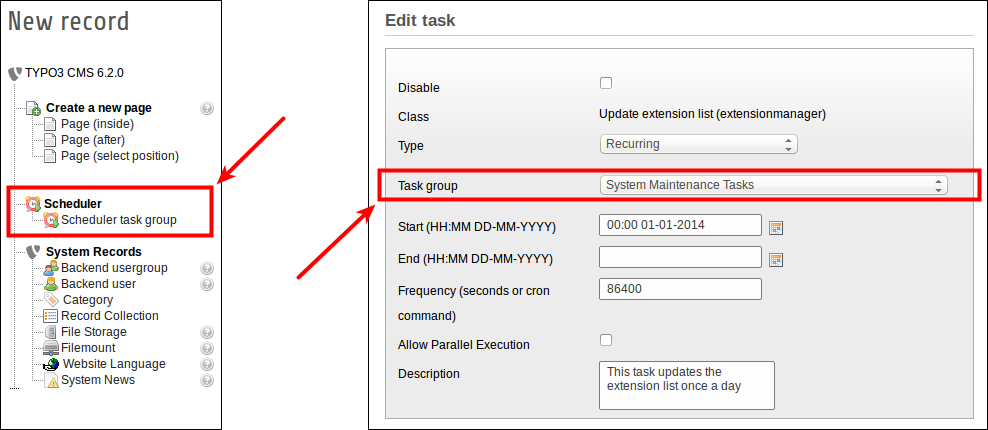
\includegraphics[width=0.85\linewidth]{Images/BackendChanges/SchedulerTaskGroup.png}
	\end{figure}

\end{frame}

% ------------------------------------------------------------------------------
% System Extension: Form
% ------------------------------------------------------------------------------
% http://forge.typo3.org/issues/38094

\begin{frame}[fragile]
	\frametitle{Backend veranderingen}
	\framesubtitle{Systeem extensie: formulieren}

	\begin{columns}[T]

		\begin{column}{.5\textwidth}
			\begin{itemize}
				\item Nieuwe post-processor vppr cObject FORM: \textbf{redirect}\newline
					(redirect na het verzenden van het formulier)
				\item Waarde wordt geparsed door \texttt{typolink} (TypoScript function),\newline
					wat betekend dat de pagina een pagina id of een URL kan zijn
					\end{itemize}
		\end{column}

		\begin{column}{.5\textwidth}
			\begin{figure}\vspace*{-0.4cm}
				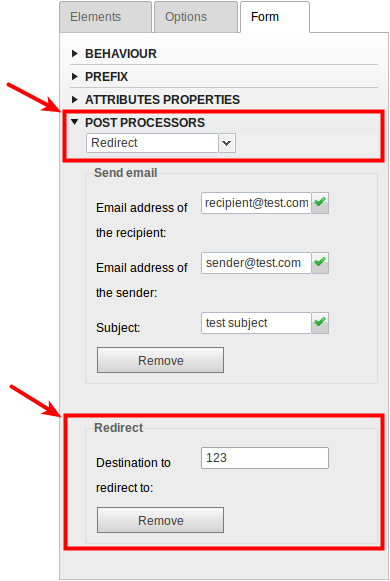
\includegraphics[width=0.65\linewidth]{Images/BackendChanges/FormRedirectPostProcessor.png}
			\end{figure}
		\end{column}

	\end{columns}

\end{frame}

% ------------------------------------------------------------------------------
% Module: List
% ------------------------------------------------------------------------------
% http://forge.typo3.org/issues/49810

\begin{frame}[fragile]
	\frametitle{Backend veranderingen}
	\framesubtitle{Lijst Module}

	\begin{itemize}
		\item Extra kolommen "UID" en "PID" in het overzicht van de lijst voor gebruikers die geen admins zijn
	\end{itemize}

	\begin{figure}
		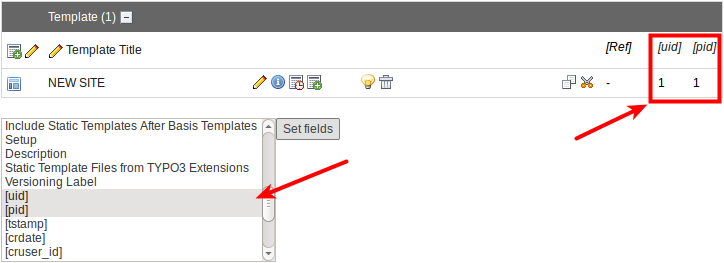
\includegraphics[width=0.95\linewidth]{Images/BackendChanges/AdditionalColumnsInListModule.png}
	\end{figure}

\end{frame}

% ------------------------------------------------------------------------------
% File Abstraction Layer
% ------------------------------------------------------------------------------
% http://forge.typo3.org/issues/50827
% http://forge.typo3.org/issues/51097

\begin{frame}[fragile]
	\frametitle{Backend veranderingen}
	\framesubtitle{File Abstraction Layer}

	\begin{itemize}
		\item Als de indexer een ontbrekend bestand vindt dan wordt een bericht getoond en een vlag in de databaserecord wordt toegevoegd. 
		\item Module "Raportages" geeft hiervan ook melding
		\item Wanneer het bestand weer wordt gevonden verdwijnen de vlag en het bericht
	\end{itemize}

	\begin{columns}[T]

		\begin{column}{.5\textwidth}
			\begin{figure}
				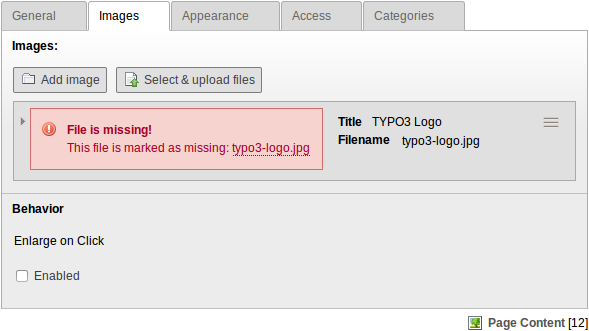
\includegraphics[width=0.95\linewidth]{Images/BackendChanges/FalMissingFileContentElement.png}
			\end{figure}
		\end{column}

		\begin{column}{.5\textwidth}
			\begin{figure}
				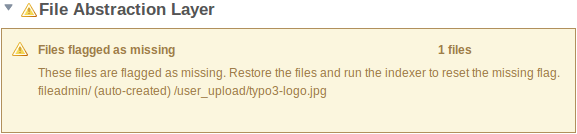
\includegraphics[width=0.95\linewidth]{Images/BackendChanges/FalMissingFileReportsModule.png}
			\end{figure}
		\end{column}

	\end{columns}

\end{frame}

% ------------------------------------------------------------------------------
% Menu/Sitemap: Categories-based Menus
% ------------------------------------------------------------------------------
% http://forge.typo3.org/issues/51161

\begin{frame}[fragile]
	\frametitle{Backend veranderingen}
	\framesubtitle{Categorie-gebasseerde menus}

	\begin{itemize}
		\item Content element "Menu/Sitemap" kan een menu creeren, gebaseerd op categorieen
			(nieuwe type van menu: "Pagina's voor geselecteerde categorie")
	\end{itemize}

	\begin{figure}
		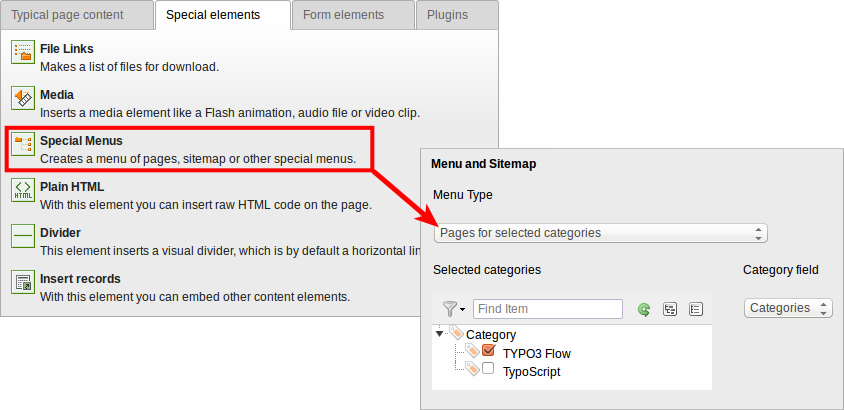
\includegraphics[width=0.8\linewidth]{Images/BackendChanges/CategoryBasedMenus.png}
	\end{figure}

\end{frame}

% ------------------------------------------------------------------------------
% Sorting Categories
% ------------------------------------------------------------------------------
% http://forge.typo3.org/issues/51590

\begin{frame}[fragile]
	\frametitle{Backend veranderingen}
	\framesubtitle{Sorteren categorieen}

 	\begin{itemize}
		\item Categorieen kunnen worden gesorteerd nu
	\end{itemize}

	\begin{figure}
		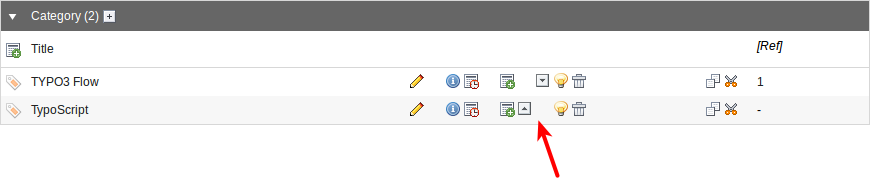
\includegraphics[width=0.95\linewidth]{Images/BackendChanges/CategorySorting.png}
	\end{figure}

\end{frame}

% ------------------------------------------------------------------------------
% Category Visibility
% ------------------------------------------------------------------------------
% http://forge.typo3.org/issues/52718

\begin{frame}[fragile]
	\frametitle{Backend veranderingen}
	\framesubtitle{Categorie Zichtbaarheid}

 	\begin{itemize}
		\item Zichtbaarheid van de categorieen kan worden beperkt voor BE gebruikers/groepen
	\end{itemize}

	\begin{figure}
		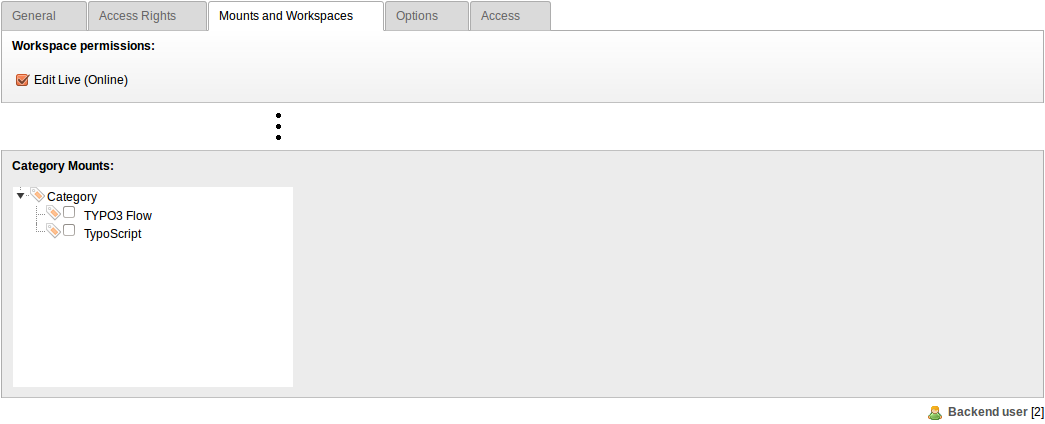
\includegraphics[width=0.95\linewidth]{Images/BackendChanges/CategoryVisibility.png}
	\end{figure}

\end{frame}

% ------------------------------------------------------------------------------
% "New Content" icon always visible
% ------------------------------------------------------------------------------
% http://forge.typo3.org/issues/48938
% http://forge.typo3.org/issues/51480

\begin{frame}[fragile]
	\frametitle{Backend veranderingen}
	\framesubtitle{Usability}

 	\begin{itemize}
		\item Icoon "nieuwe content" is altijd zichtbaar wanneer de kolom leeg is
			(dit helpt editors te begrijpen wat ze kunnen doen)
	\end{itemize}

	\begin{figure}
		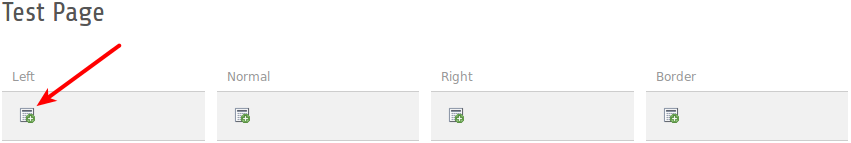
\includegraphics[width=0.95\linewidth]{Images/BackendChanges/NewContentIconAlwaysVisible.png}
	\end{figure}

\end{frame}

% ------------------------------------------------------------------------------
% Module "Functions": Hide In Menus
% ------------------------------------------------------------------------------
% http://forge.typo3.org/issues/51017

\begin{frame}[fragile]
	\frametitle{Backend veranderingen}
	\framesubtitle{Functies}

 	\begin{itemize}
		\item Wanneer je meerdere pagina's aanmaakt in de module "Functies"\newline
			is er een nieuwe checkbox welke gebruikers het toestaat deze paginas \newline
			te verbergen in het menu
		\item Erg handig wanneer je meerdere paginas tegelijk aanmaakt. 
	\end{itemize}

	\begin{figure}
		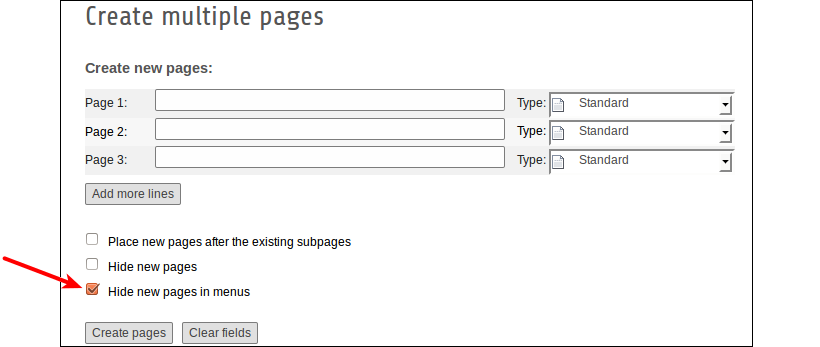
\includegraphics[width=0.85\linewidth]{Images/BackendChanges/CreateMultiplePagesHideInMenu.png}
	\end{figure}

\end{frame}

% ------------------------------------------------------------------------------
% Extension Manager: Upload Extensions
% ------------------------------------------------------------------------------
% http://forge.typo3.org/issues/51776
% http://forge.typo3.org/issues/51437

\begin{frame}[fragile]
	\frametitle{Backend veranderingen}
	\framesubtitle{Extensiemanager}

 	\begin{itemize}
		\item Je kan een extensie uploaden via de "Get Extensions" functie
	\end{itemize}

	\begin{figure}
		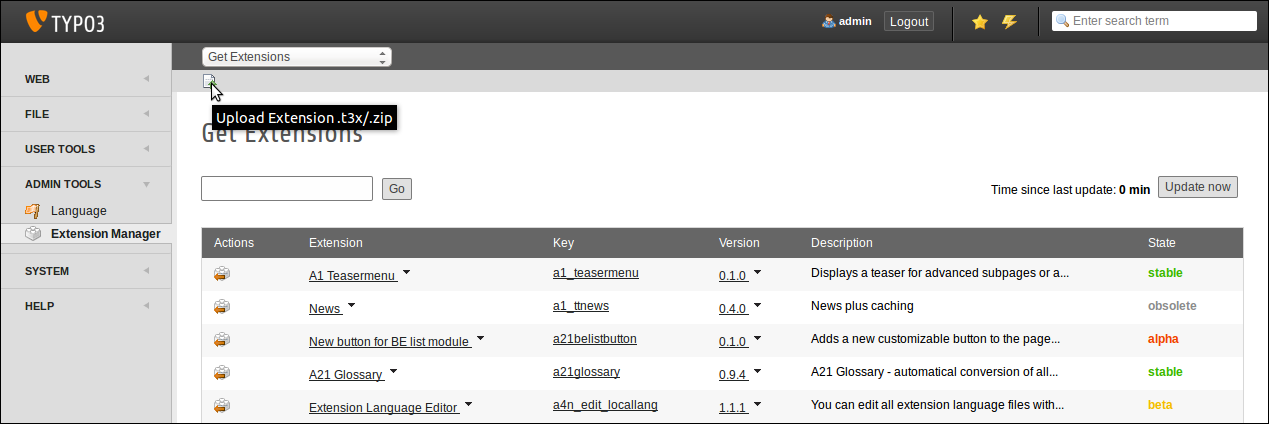
\includegraphics[width=0.95\linewidth]{Images/BackendChanges/UploadExtension.png}
	\end{figure}

\end{frame}

% ------------------------------------------------------------------------------
% Recycler
% ------------------------------------------------------------------------------
% http://forge.typo3.org/issues/52324

\begin{frame}[fragile]
	\frametitle{Backend veranderingen}
	\framesubtitle{Prullenbak}

 	\begin{itemize}
		\item De prullenbak records kunnen worden gesorteerd op timestamp (tstamp)\newline
			(dit helpt gebruikers bij het beslissen om een bepaald record terug te zetten)
	\end{itemize}

	\begin{figure}
		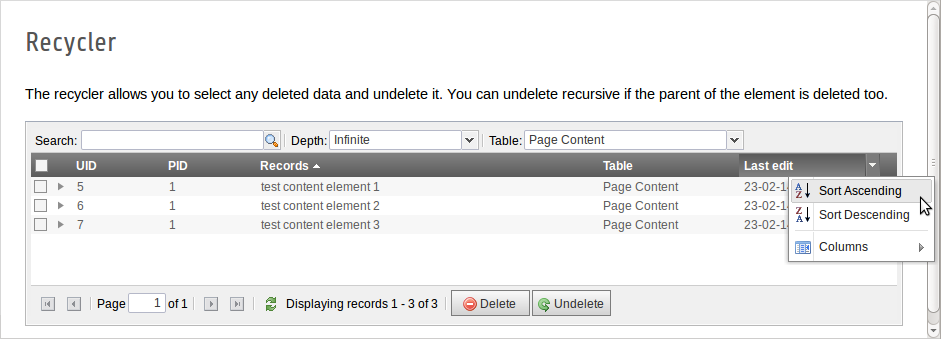
\includegraphics[width=0.95\linewidth]{Images/BackendChanges/RecyclerSortRecord.png}
	\end{figure}

\end{frame}

% ------------------------------------------------------------------------------
% File/Directory Permissions
% ------------------------------------------------------------------------------

\begin{frame}[fragile]
	\frametitle{Backend veranderingen}
	\framesubtitle{Bestand/mappen permissies}

 	\begin{itemize}
		\item Nog meer uitgebreide bestand/mappen permissies voor BE gebruikers/groepen
			\begingroup\color{typo3red}\textbf{(1)}\endgroup
		\item Dit is mogelijk sinds TYPO3 6.0, alleen via UserTSconfig
			\begingroup\color{typo3red}\textbf{(2)}\endgroup
	\end{itemize}

	\begin{figure}
		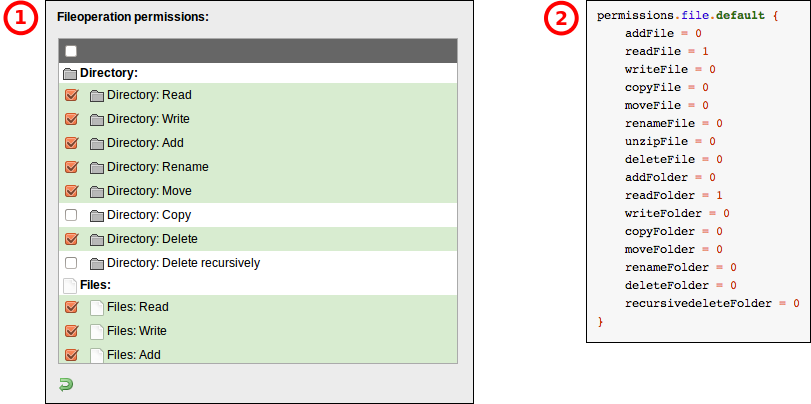
\includegraphics[width=0.75\linewidth]{Images/BackendChanges/FileAndDirectoryPermissions.png}
	\end{figure}

\end{frame}

% ------------------------------------------------------------------------------
% OpenID
% ------------------------------------------------------------------------------

\begin{frame}[fragile]
	\frametitle{Backend veranderingen}
	\framesubtitle{OpenID (1)}

 	\begin{itemize}
		\item OpenID voor BE gebruikers authenticatie kan worden \newline 
		geconfigureerd door middel van een wizard
		\item EXT:openid (systeem extensie) is nodig voor deze feature
	\end{itemize}

	\begin{figure}
		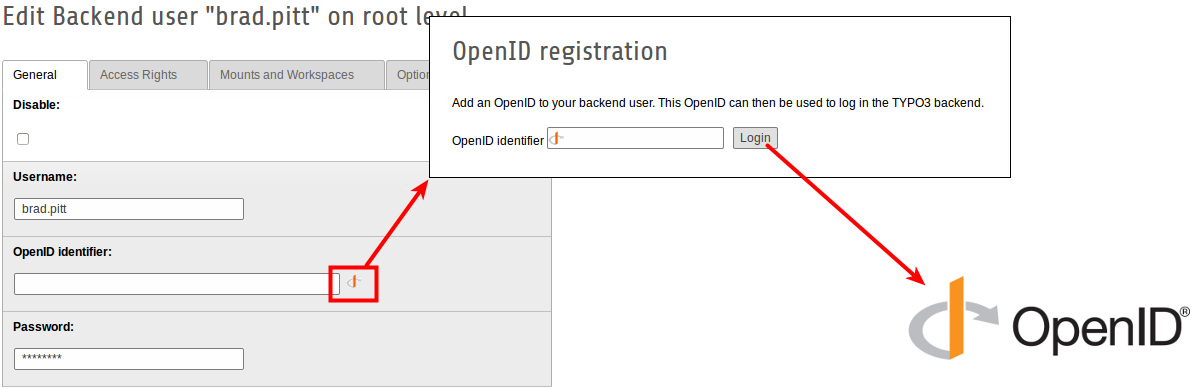
\includegraphics[width=0.95\linewidth]{Images/BackendChanges/OpenIdWizard.png}
	\end{figure}

\end{frame}

% ------------------------------------------------------------------------------
% OpenID
% ------------------------------------------------------------------------------

\begin{frame}[fragile]
	\frametitle{Backend veranderingen}
	\framesubtitle{OpenID (2)}

 	\begin{itemize}
		\item OpenID voor BE gebruikers authenticatie kan worden \newline 
		geconfigureerd door middel van een wizard
		\item EXT:openid (systeem extensie) is nodig voor deze feature
	\end{itemize}

	\begin{figure}
		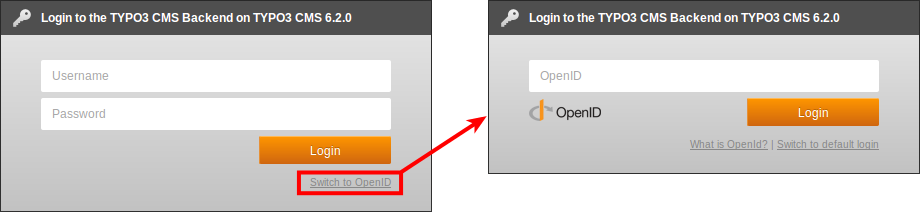
\includegraphics[width=0.8\linewidth]{Images/BackendChanges/OpenIdLogin.png}
	\end{figure}

 	\begin{itemize}
		\item Further details about OpenID:\newline
			\small\url{http://openid.net}\normalsize
	\end{itemize}

\end{frame}

% ------------------------------------------------------------------------------
% Workspaces
% ------------------------------------------------------------------------------
% http://forge.typo3.org/issues/50223
% http://forge.typo3.org/issues/50224

\begin{frame}[fragile]
	\frametitle{Backend veranderingen}
	\framesubtitle{Workspaces}

 	\begin{itemize}
		\item Editors/gebruikers kunnen aangeven wie een notificatie krijgt \newline 
		zonder dat dit kan worden gelimiteerd op systeemlevel
		\item Tab "All" is nu zichtbaar voor \underline{alle} gebruikers
	\end{itemize}

	\begin{figure}
		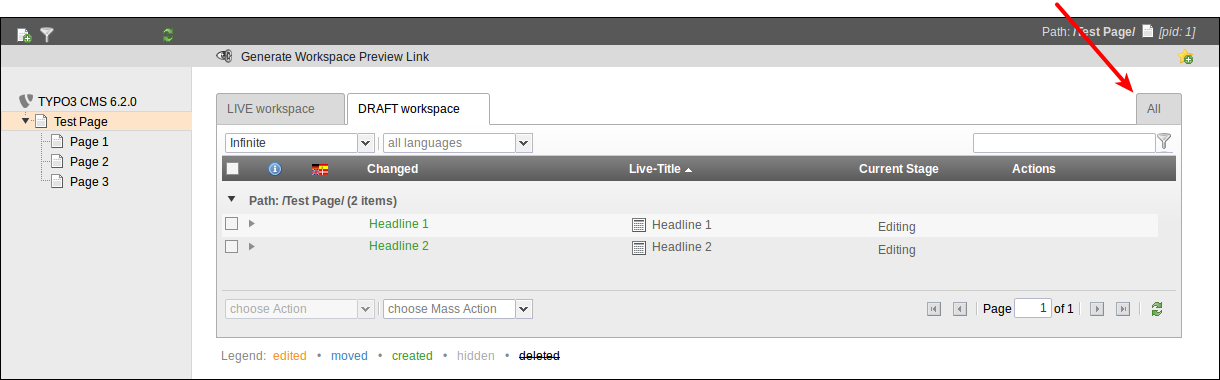
\includegraphics[width=0.95\linewidth]{Images/BackendChanges/WorkspacesTabAll.png}
	\end{figure}

\end{frame}

% ------------------------------------------------------------------------------

